%standard 3.2

%start_of_questions

%new_question
%%%%%%%%%%%%%%%%%%%%%
	% Problem 5
	% Difficulty: 2
%%%%%%%%%%%%%%%%%%%%%
	\item  
		Write a program that prompts the user to enter three integers and displays the integers 
		in increasing order (smallest to largest).  You may not use the built-in functions 
		\textit{max}(), \textit{min}(), \textit{sort}() or \textit{sorted}().


%new_question
%%%%%%%%%%%%%%%%%%%%%
	% Problem 6
	% Difficulty: 2
%%%%%%%%%%%%%%%%%%%%%
	\item  
		Write a program that prompts the user to enter three integers and displays the integers 
		in decreasing order (largest to smallest).  You may not use the built-in functions 
		\textit{max}(), \textit{min}(), \textit{sort}() or \textit{sorted}().


%new_question
%%%%%%%%%%%%%%%%%%%%%
	% Problem 7
	% Difficulty: 2
%%%%%%%%%%%%%%%%%%%%%
	\item  
		In Harry Potter, the currency consists of knuts, sickle, and galleon.  There are 29 knuts in 
		one sickle and 17 sickles in one galleon.  Write a program that will convert some amount of 
		knuts into the fewest amount of coins possible.  Only print non-zero values, meaning don't 
		print something similar to ``0 sickles.''  For example,
		\begin{itemize}
			\item Given 32 knuts, output 1 sickle 3 knuts
			\item Given 544 knuts, output 1 galleon 4 sickles 18 knuts
			\item Given 993 knuts, output 2 galleons 7 knuts. 
				Do \textbf{not} output 2 galleons 0 sickle 7 knuts.
		\end{itemize}




%new_question
%%%%%%%%%%%%%%%%%%%%%
	% Problem 12
	% Difficulty: 2
%%%%%%%%%%%%%%%%%%%%%
	\item  
		%https://edabit.com/challenge/b8wRDMWgMZTN2nmfx
		Ask the user for three integers.  Determine (and output) how many copies of the same number 
		the user entered.\\
		For example, \\ \ \hfill
		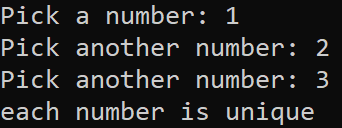
\includegraphics[height = 0.6in]{./imgs/uniqueIntCount1.PNG} \hfill
		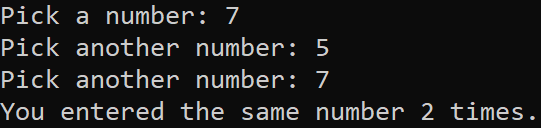
\includegraphics[height = 0.6in]{./imgs/uniqueIntCount2.PNG} \hfill \ 

	
%new_question
%%%%%%%%%%%%%%%%%%%%%
	% Problem 13
	% Difficulty: 2
%%%%%%%%%%%%%%%%%%%%%
	\item  
		Primary U.S. interstate highways are numbered 1-99.  Odd numbers (like 5 or 95) go north/
		south, and evens (like 10 or 82) go east/west.  Auxiliary highways are numbered 100-999, and 
		service the primary highway indicated by the rightmost two digits.  Thus, I-405 services 
		I-5, and I-290 services I-90.
		
		Note: 200 is not a valid auxiliary highway because 00 is not a valid primary highway 
		number.\\
		
		Let the user pick a highway number.  Given a valid highway number, indicate whether it runs 
		north/south or east/west.  If it is an invalid highway number, indicate that it is an 
		invalid highway number. \\
		For example,
		
		\hfill
		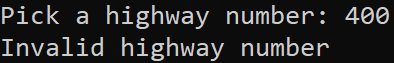
\includegraphics[width = 2in]{./imgs/highwayValidator1.PNG} \hfill
		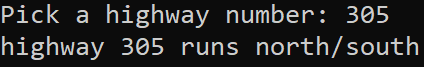
\includegraphics[width = 2in]{./imgs/highwayValidator2.PNG} \hfill \ 

		\hfill 
		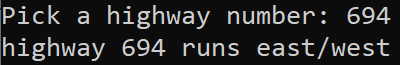
\includegraphics[width = 2in]{./imgs/highwayValidator3.PNG} \hfill 
		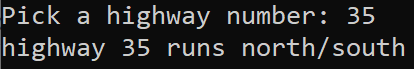
\includegraphics[width = 2in]{./imgs/highwayValidator4.PNG} \hfill \ 



%new_question
%%%%%%%%%%%%%%%%%%%%%
	% Problem 17
	% Difficulty: 2
%%%%%%%%%%%%%%%%%%%%%
	\item  
		%https://edabit.com/challenge/sfqudQHQ3HPpd7dZb
		Create a game of Rock, Paper, Scissors that takes user inputs.  
		The first input should be player 1 and the second 
		input should be player 2.  Print the winner according to the following rules. 
		\begin{itemize}
			\item Rock beats Scissors
			\item Scissors beats Paper
			\item Paper beats Rock
		\end{itemize}		
		For example:

		\hfill 
		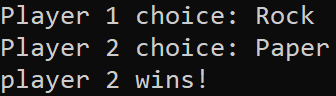
\includegraphics[height = 0.5in]{./imgs/RockPaperScissors1.PNG} \hfill 
		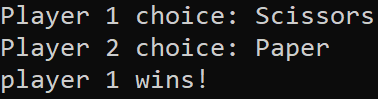
\includegraphics[height = 0.5in]{./imgs/RockPaperScissors2.PNG} \hfill  
		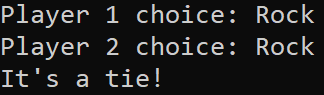
\includegraphics[height = 0.5in]{./imgs/RockPaperScissors3.PNG} \hfill \ 


%new_question
%%%%%%%%%%%%%%%%%%%%%
	% Problem 18
	% Difficulty: 2
%%%%%%%%%%%%%%%%%%%%%
	\item  
		%https://edabit.com/challenge/ancAxGEF9MsLWXDqe
		Write a program that asks the user for three side lengths of a triangle, and prints 
		the type of triangle.  The types of triangles are 
		\begin{itemize}
			\item No sides equal: \csq{scalene}
			\item Two sides equal: \csq{isosceles}
			\item All sides equal: \csq{equilateral}	
		\end{itemize}
		For example:

		\hfill 
		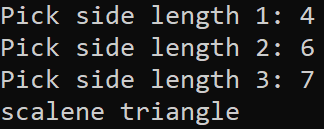
\includegraphics[height = 0.7in]{./imgs/typeOfTriangle1.PNG} \hfill 
		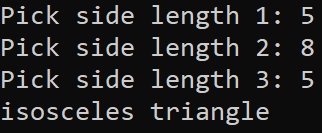
\includegraphics[height = 0.7in]{./imgs/typeOfTriangle2.PNG} \hfill  
		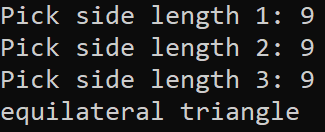
\includegraphics[height = 0.7in]{./imgs/typeOfTriangle3.PNG} \hfill \ 




%end_of_questions








